\subsect{Sprint 5}{sprint5}

\underline{Fecha de inicio}: 11/10/2022

\underline{Fecha de fin}: 11/11/2022

\underline{Objetivos}:
\begin{itemize}
	\item Completar la migración al servidor personal.
	\item Nuevo sistema de menciones.
\end{itemize}

\underline{Descripción}:
En este sprint se añadirá la funcionalidad de menciones, de forma que se pueda mencionar a un usuario en un
mensaje y que este reciba una notificación.\ Además, se completará la migración de la aplicación al servidor
personal.\ Los correos electrónicos que reciben los usuarios se enviarán sin utilizar ningún servicio externo,
ya que hay ocasiones en que ciertos servicios de correo electrónico bloquean los correos que se envían desde
estas plataformas, como SendGrid.\ Debido a esto, se ha creado una cuenta de correo electrónico en Gmail, con el nombre
de la aplicación, y se utilizará para enviar los correos electrónicos.

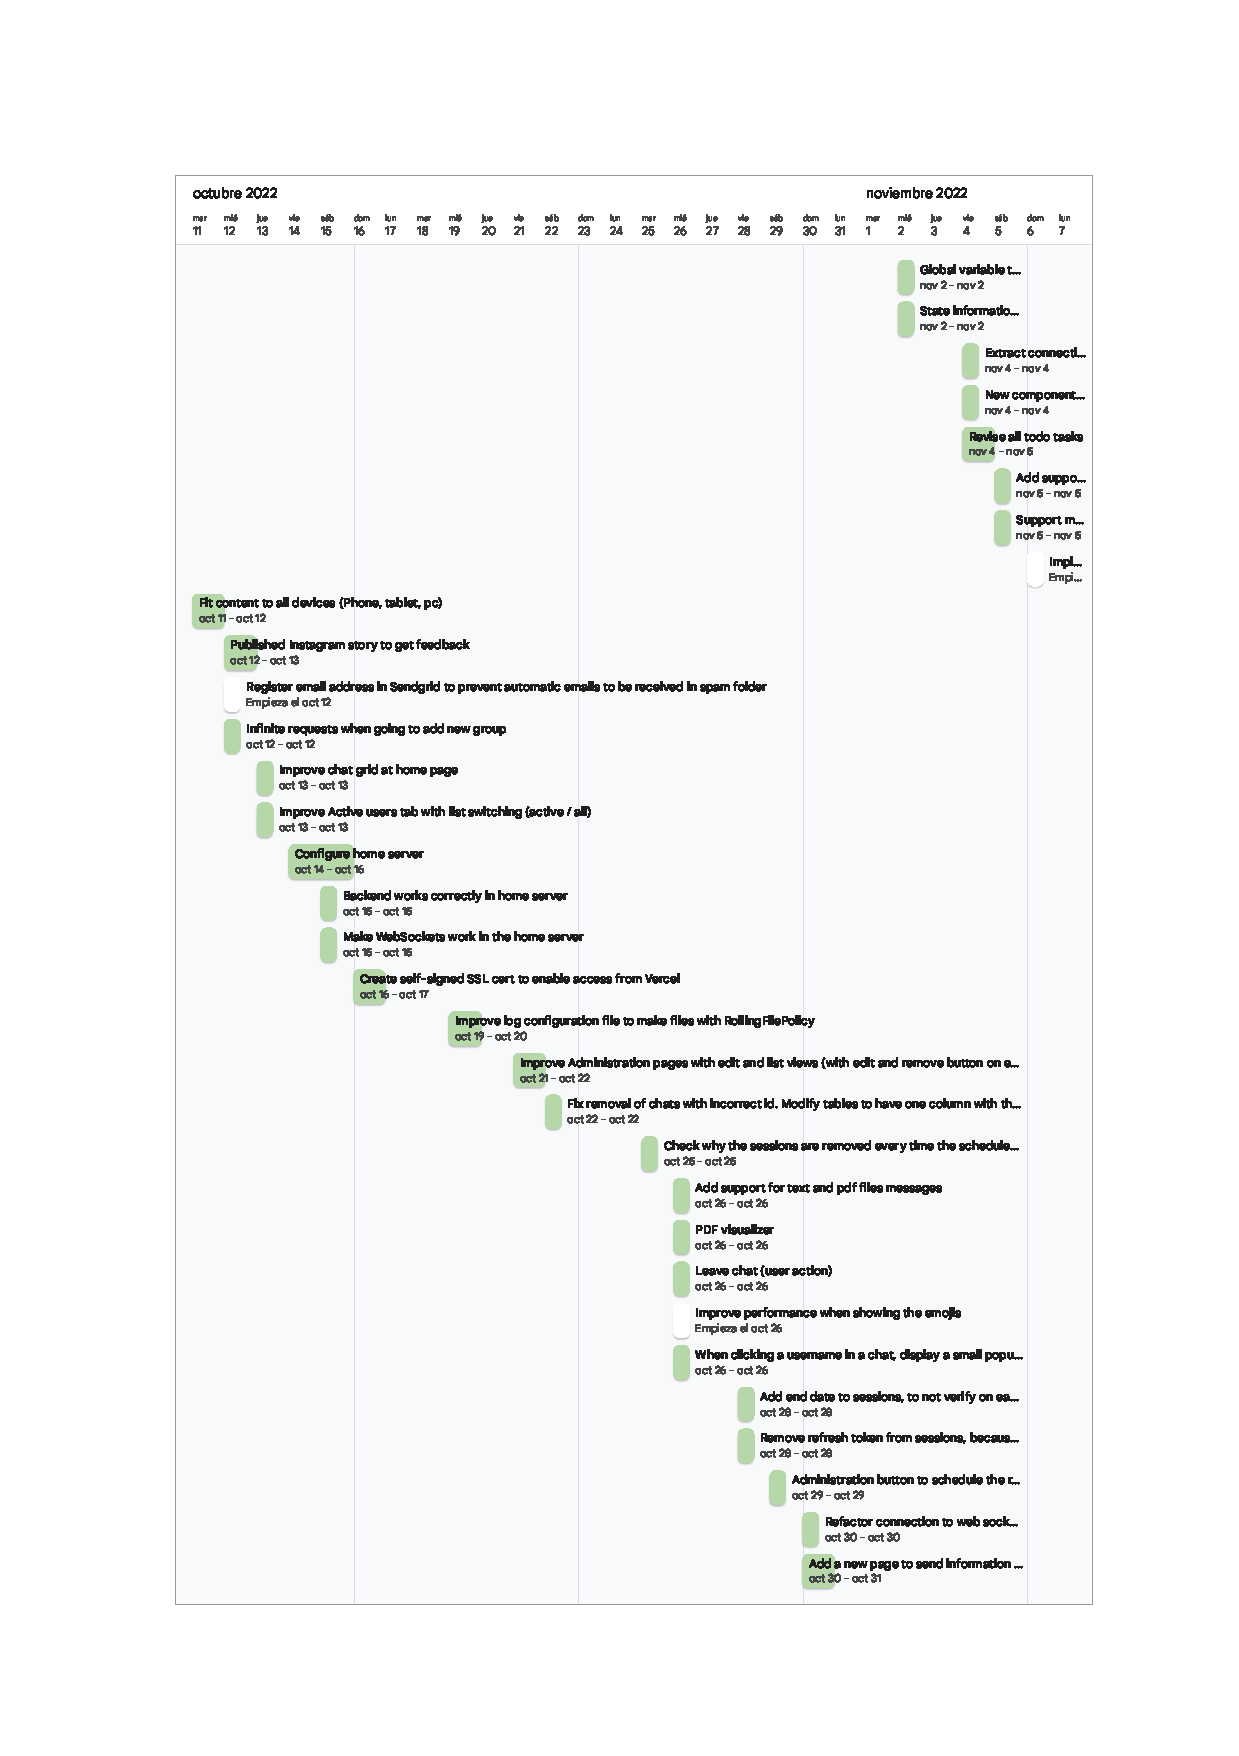
\includepdf[pages=-]{backlog/sprints/Sprint5.pdf}
